\documentclass[report]{nrel}

\usepackage[latin1]{inputenc}
\usepackage{amsmath}
\usepackage{amsfonts}
\usepackage{amssymb}
\usepackage{graphicx}
\usepackage{units}
\usepackage{moreverb}
\usepackage{siunitx}  %RRD
\sisetup{group-separator = {,}} %RRD
\DeclareSIUnit\year{yr}
\DeclareSIUnit\nmi{nmi}

\usepackage[
nonumberlist, %do not show page numbers
acronym,      %generate acronym listing
toc,          %show listings as entries in table of contents
section,      %use section level for toc entries
nomain]       %No main glossary 
{glossaries}

\usepackage{hyperref}
\urlstyle{rm} %RRD to put url in roman

\usepackage{array}          %RRD to help with table wrapping
\usepackage[flushleft]{threeparttable}       %RRD to help with tablenotes
\usepackage{tabularx,tabulary,longtable}       %RRD to help with table wrapping
\usepackage{multirow}       %RRD to help with table wrapping
\usepackage{textcomp} %RRD trademark
\usepackage{amsfonts}    %RRD to help with some math fonts

\renewcommand{\vec}[1]{\underline{#1}}

\graphicspath{../PICS/}     %RRD PICS folder path                             
%\usepackage[caption=false]{subfigure}


\newcommand\BibTeX{{\rmfamily B\kern-.05em \textsc{i\kern-.025em b}\kern-.08em
		T\kern-.1667em\lower.7ex\hbox{E}\kern-.125emX}}

%\usepackage[square]{natbib} %RRD
%\bibliographystyle{abbrvnat}
%\setcitestyle{authoryear, open={[(},close={)]}}


%Generate a list of symbols (acronyms are a default glossary)
%            log    name        in  out   title
\newglossary[syl]{symbolslist}{syi}{syo}{List of Symbols}
\newglossary[gkl]{greek}{kls}{klo}{Greek Symbols}

%Remove the dot at the end of glossary descriptions
\renewcommand*{\glspostdescription}{}

\let\firstchar\lowercase
\let\oldprintglossary\printglossary
\def\printglossary{\let\firstchar\uppercase\oldprintglossary}

% a bigger glossary description width:
\setlength\glsdescwidth{.9\textwidth}

%Activate glossary commands
\makeglossaries

%These commands sort the lists
%makeindex -s DynStall.ist -t DynStall.alg -o DynStall.acr DynStall.acn
%makeindex -s DynStall.ist -t DynStall.glg -o DynStall.gls DynStall.glo
%makeindex -s DynStall.ist -t DynStall.syl -o DynStall.syi DynStall.syo
\usepackage{glossary-mcols}
\setglossarystyle{mcolindex}


\def\ie{i.e., }
\def\eg{e.g., }
\def\cf{cf., }
\loadglsentries{glossary}

\makeglossaries
% \makenoidxglossaries

\def\ie{i.e.,}
\def\eg{e.g.,}
\def\cosa{\ensuremath{\cos{\alpha}}}
\def\sina{\ensuremath{\sin{\alpha}}}

\author{Rick Damiani}
\title{Theory Base for KiteAeroDyn}

\addbibresource{C:/users/rdamiani/dropbox/references.bib}


\begin{document}
\glsdisablehyper

\frontmatter
\setcounter{page}{4}
\chapter*{Executive Summary}
This manual summarizes the theory and preliminary verifications of the \gls{vsm} module (\gls{kitevsm}), which is part of \gls{kitead}, the new aerodynamics module of \gls{kitefast} for airborne wind energy. SOMETHING ABOUT THEORY AND VERIFICATION HERE. The results are encouraging, and future improvements to the code are recommended in this manual. 
%_______________________________________ %
\chapter*{Acknowledgments}
This work was supported by Makani Google X  under Contract No. with the National Renewable Energy Laboratory. 
%_______________________________________ %

\glsresetall


\tableofcontents

\listoffigures
\listoftables
\section*{\Large{List of Acronyms and Symbols}}\label{sec:symbols}
%\addcontentsline{toc}{section}{\nameref{sec:symbols}}%
\printglossary[type=\acronymtype,style=long]
\printglossary[type=symbols,style=long, title=Symbols]
\printglossary[type=greek,style=long, title=Greek Symbols]
\let\firstchar\lowercase %Reset to lowercase this command

\mainmatter
\lstset{language=[LaTeX]Tex,columns=fullflexible,keepspaces=true,breaklines=true}

%\maketitle


%\footnotetext[2]{Please ensure that you use the most up to date

%____________________________________________________________ %
\chapter{Overview}\label{sec:overview}
	
	The dynamics of semi-rigid kites can be simulated by combining  models for aerodynamics and structures. This manual describes the theory developed and implemented in \gls{kitead}, a new aerodynamics module that works within the \gls{mbdyn} framework to simulate airborne wind energy kites.
	
	The main aerodynamic problem for aircraft-like structures winds down to solving for the induction associated with the vorticity field generated by the presence of lifting surfaces. In this document we will call lifting surfaces `wings', regardless of the actual component function of the surfaces.  Various methods exist to accomplish this task, and with various levels of fidelity and computational demand.  \Gls{kitevsm} is based on Weissenger's method \citep{weissinger1947}, also known as \glsentrydesc{vsm} (\gls{vsm}), but with some modifications and extensions to improve the accuracy, computational efficiency, minimization of instabilities and to include the nonlinear airfoil polar data and multiple lift surface contributions.
	
	
%___________________________________________________________________________________________ %
\section{\glsentrytext{vsm} Theory Development}\label{sec:theory}
The \gls{vsm} belongs to the vortex-lattice class, and it approximates Prandtl's lifting line theory \citep{prandtl1918}, with contributions from the work of Munk \citep[stagger theorem][]{munk1921}, Pistolesi \citep[$\nicefrac{3}{4}$-chord theorem]{pistolesi1929},Wieghardt \citep{wieghardt1940}, and Mutterperl \citep{mutterperl1941}. 
The lifting-line method can be applied to straight, planar wings of high aspect ratio (\gls{ar}>4). In its original formulation, this method reaches a closed form solution for the induced angle of attack along the wing span by assuming a simple flat plate behavior, where the lift coefficient is simply regarded as $\gls{cl}=2\pi\gls{aoa}$. 

The \gls{vsm}, on the other hand, promises accurate solutions for low and high \glspl{ar} wings of different shape, including swept and dihedral wings. Furthermore, the \gls{vsm} can be modified to account for the nonlinear polar curve of real airfoils.

Whereas Pradtl's lifting line sheds a continuous trailing vorticity from the wing's $\nicefrac{1}{4}$-chord line, the \gls{vsm} approximates the resulting vortex-sheet with a finite number of horseshoe vortices. The bound portion of the horseshoe vortex lies along the \gls{14c} line, with the trailing arms aligned with the freestream direction. 
%TO DO: MAKE SURE WE FINALIZE DIRECTION OF VORTICES
One other difference is in the control point locations. The lifting-line calculates induction along control points at the \gls{14c}, whereas the \gls{vsm} places control points at the \gls{34c}, but in the direction of the freestream.
%TO DO: MAKE SURE WE FINALIZE DIRECTION OF CTRL POINTS

\begin{figure}[h]
	\centering
	\includegraphics[width=0.8\linewidth]{PICS/vsm01}
	\caption{Horseshoe vortices distributed following the convention of the \gls{vsm} adopted. \gls{A}, \gls{B} are the generic start and end point of the \gls{14c}-bound segment of the generic horseshoe vortex. \gls{ctlp} is a generic control point located at the \gls{34c}.}
	\label{fig:vsm_vortices}
\end{figure}
%

Normally, techniques based on Weissenger's method assumes either a simple array of unknown values or some Fourier modal representation with unknown coefficients for the circulation (\gls{circy}=\gls{circtht}). To attain the unknowns, those methods impose a slip, non-penetration wall condition at the \gls{34c} control points, which translates into solving the resulting linear system of equations. The choice of the \gls{34c} condition derives from Pistolesi's theorem, which states that the 0-lift angle of attack is approximated by the tangent to the camber line at the \gls{34c} location. Therefore, the incidence angle at the \gls{34c} point is equal to $\gls{aoainc}=\gls{aoag}-\arctan\left( \left. \frac{dx}{dy} \right|_\mathrm{\gls{34c}} \right)$ (assuming an airfoil local reference frame).
%
\begin{figure}[h]
	\centering
	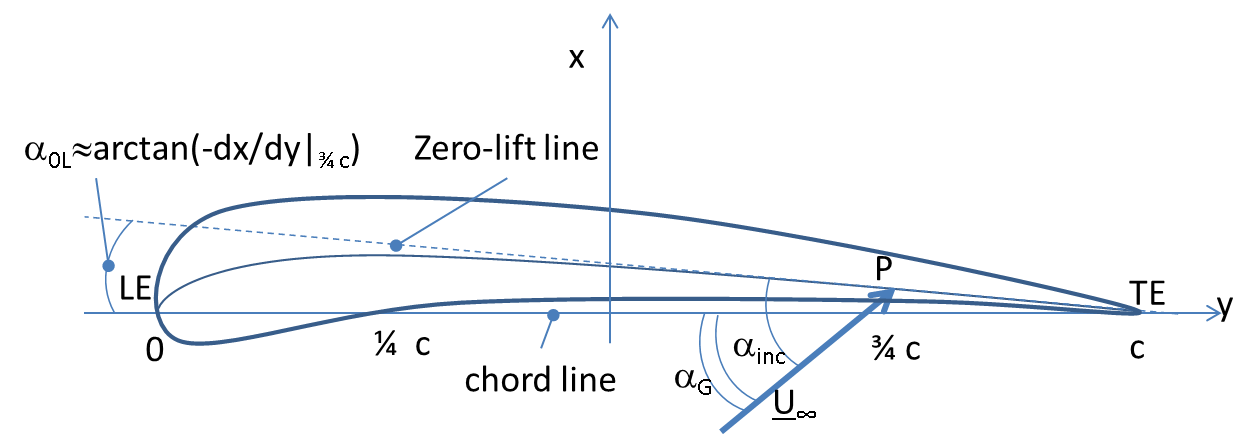
\includegraphics[width=0.8\linewidth]{PICS/pistolesi}
	\caption{Representation of Pistolesi's theorem at the generic spanwise wing section. Note the local airfoil coordinate system is displayed.}
	\label{fig:pistolesi}
\end{figure}
%

The induced velocity at the \glsentrydesc{ctlpj} (\gls{ctlpj}) can be obtained by summing the contributions from all horseshoe vortices with associated circulation \gls{circvi}. The generic induced velocity by the \emph{i-th} horseshoe vortex (\gls{ab}, \gls{ainf}, \gls{binf}) of circulation \gls{circvi} on the generic \gls{ctlpj} can be written, with reference to Fig.~\ref{fig:vsm_vortices} and ~\ref{fig:inducedvel}, as in Eq.~\eqref{eq:inducedvel}:
%
\begin{equation}\label{eq:inducedvel}
\gls{uindvij} =\gls{uabv} + \gls{uainfv} +  \gls{ubinfv}
\end{equation}
%
where \gls{uindvij} is the \glsentrydesc{uindvij}; \gls{uabv} is the \glsentrydesc{uabv} ; \gls{uainfv} is the \glsentrydesc{uainfv}; \gls{ubinfv} is the \glsentrydesc{ubinfv}.
%
\begin{figure}[h]
	\centering
	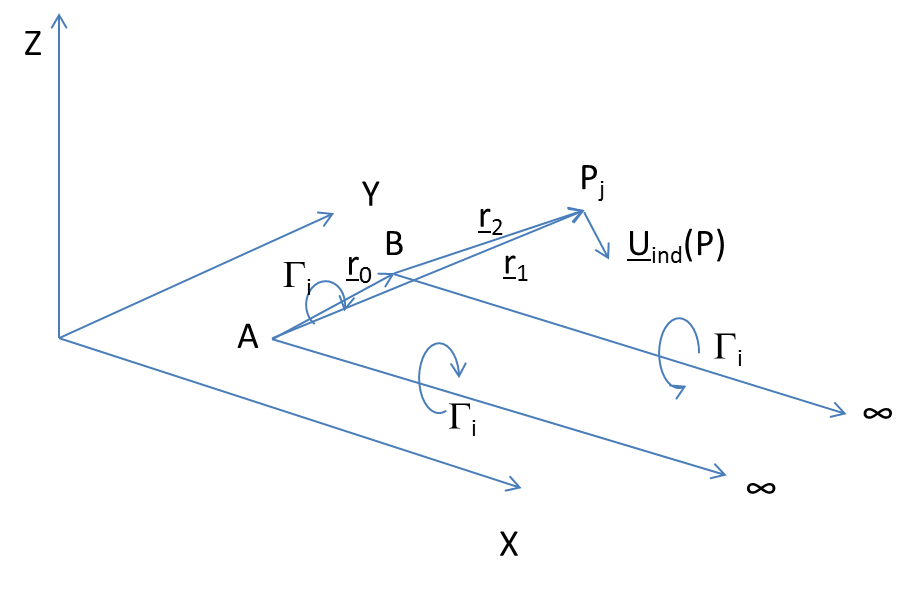
\includegraphics[width=0.8\linewidth]{PICS/inducedvel}
	\caption{Contribution of the generic \emph{i-th} horseshoe vortex to the induced velocity at the generic \gls{ctlpj}.}
	\label{fig:inducedvel}
\end{figure}
%

The various terms in Eq.~\eqref{eq:inducedvel} can be found by using the Biot-Savart law and can be expressed \citep[ref.][]{phillips2000} as in Eq.~\eqref{eq:3dindvel}:
%
\begin{equation}\label{eq:3dindvel}
	\renewcommand*{\arraystretch}{2.5}
	\begin{array}{lcl}
		\gls{uabv}  &=& \left\{\begin{array}{lr}
		\dfrac{\gls{circi}}{4\pi} \dfrac{\gls{r1} \times \gls{r2}}{\left| \gls{r1} \times \gls{r2}  \right|^2} \left[\gls{r0} \cdot \left( \dfrac{\gls{r1}}{\gls{r1m}} - \dfrac{\gls{r2}}{\gls{r2m}} \right) \right]
		& \mathrm{if }\quad \dfrac{\left|\gls{r1} \times \gls{r0}\right|}{\gls{r0m}} > \gls{epscore2} \\
		
		\dfrac{\left|\gls{r1} \times \gls{r0}\right|} {\gls{r0m}\gls{epscore2}}\gls{uabvpp} & \mathrm{otherwise} 
		
		\end{array} \right. \\
		
		\gls{uainfv} &=& \left\{
		\begin{array}{lr}
			 \dfrac{\gls{circi}}{4\pi} \dfrac{1 + \dfrac{\gls{r1} \cdot \gls{xiv}}{\gls{r1m}} } {\left| \gls{r1} \times \gls{xiv} \right|^2} \gls{r1} \times \gls{xiv} & \mathrm{if }\quad \left|\gls{r1} \times \gls{xiv} \right| > \gls{epscore} \\

			 \dfrac{\left|\gls{r1} \times \gls{xiv}\right|}{\gls{epscore}}\gls{uainfvpp} & \mathrm{otherwise}  \\

		  \end{array} \right .\\
		 
		\gls{ubinfv} &=& \left\{
		\begin{array}{lr}
			-\dfrac{\gls{circi}}{4\pi} \dfrac{1 + \dfrac{\gls{r2} \cdot \gls{xiv}}{\gls{r2m}} } {\left| \gls{r2} \times \gls{xiv} \right|^2} \gls{r2} \times \gls{xiv}  & \mathrm{if }\quad \left|\gls{r2} \times \gls{xiv} \right| > \gls{epscore} \\
			
			\dfrac{\left|\gls{r2} \times \gls{xiv}\right|}{\gls{epscore}}\gls{ubinfvpp} & \mathrm{otherwise}  \\
		
		\end{array} \right .\\
		
\end{array}
\end{equation}
% 
where \gls{r0} is the \glsentrydesc{r0}; \gls{r1} is the \glsentrydesc{r1}; \gls{r2} is the \glsentrydesc{r2}; and \gls{xiv} is the \glsentrydesc{xiv}; the vortex core radius \gls{epscore} for the trailing vorticity is given by Eq.~\eqref{eq:epscore} \citep{bhagwat2002} (see also Figure~\ref{fig:epscore1}):
%
\begin{equation}\label{eq:epscore}
\gls{epscore}=\sqrt{4\gls{oseen}\gls{airvisc}\dfrac{\left|\gls{rpn}\right|}{\gls{uoo}}}
\end{equation}
%
where \gls{airvisc} is the \glsentrydesc{airvisc}; \gls{oseen} is the \glsentrydesc{oseen}; and \gls{rpn} is the \glsentrydesc{rpn} as shown in Eq.\eqref{eq:rpn}:
%
\begin{equation}\label{eq:rpn}
\gls{rpn}= (\gls{rgen} \cdot \gls{xiv}) \gls{xiv}
\end{equation}
%
where \gls{rgen} is the \glsentrydesc{rgen}.
%
\begin{figure}[h]
	\centering
	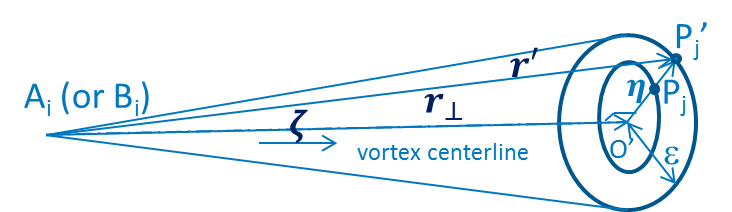
\includegraphics[width=0.5\linewidth]{PICS/epscore1}
	\caption{Diagram showing the relative location of of \gls{A}, \gls{B}, \gls{ctlpj}, \gls{ctlppj} for the trailing-vortex core correction. Other symbols defined in the text.}
	\label{fig:epscore1}
\end{figure}
%

\gls{uainfvpp} and \gls{ubinfvpp} are the \glsentrydesc{uainfvpp}, \glsentrydesc{uainfvpp}, respectively, which can be calculated as in Eq.~\eqref{eq:uabinfvpp}:
%
\begin{equation}\label{eq:uabinfvpp}
	\renewcommand*{\arraystretch}{2.5}
\begin{array}{lcl}
	\gls{uainfvpp} & = &
\dfrac{\gls{circi}}{4\pi} \dfrac{1 + \dfrac{\gls{r1p} \cdot \gls{xiv}}{\gls{r1pm}} } {\left| \gls{r1p} \times \gls{xiv} \right|^2} \gls{r1p} \times \gls{xiv} \\
	\gls{ubinfvpp} & = &
-\dfrac{\gls{circi}}{4\pi} \dfrac{1 + \dfrac{\gls{r2p} \cdot \gls{xiv}}{\gls{r2pm}} } {\left| \gls{r2p} \times \gls{xiv} \right|^2} \gls{r2p} \times \gls{xiv} \\
\mathrm{with} & \gls{rgenp} = \gls{rpn} + \gls{epscore} \gls{corerad}
\end{array} 
\end{equation}
%
where the \gls{rgenp} is the \glsentrydesc{rgenp} (\ie~either \gls{r1p} or \gls{r2p}), and the radial unit vector \gls{corerad} can be calculated as in Eq.~\eqref{eq:corerad}:
%
\begin{equation}\label{eq:corerad}
\gls{corerad} = \dfrac{ \dfrac{\gls{rgen}}{\left|\gls{rgen}\right|} - \gls{xiv}}{\left| \dfrac{\gls{rgen}}{\left|\gls{rgen}\right|} - \gls{xiv} \right|}
\end{equation}
%

For the bound vorticity the core radius is fixed as shown in Eq.~\eqref{eq:epscore2} \citep{vangarrel2003} and Figure.~\ref{fig:epscore2}:
%
\begin{figure}[h]
	\centering
	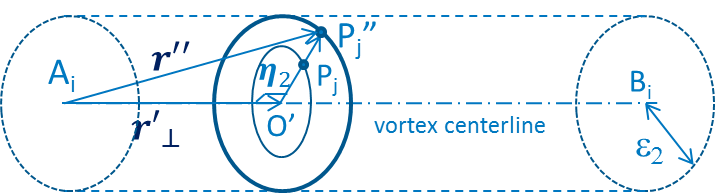
\includegraphics[width=0.5\linewidth]{PICS/epscore2}
	\caption{Diagram showing the relative location of \gls{A}, \gls{B}, \gls{ctlpj}, and \gls{ctlpppj} for the bound-vortex core correction. Other symbols defined in the text.}
	\label{fig:epscore2}
\end{figure}
%
%
\begin{equation}\label{eq:epscore2}
\gls{epscore2}=0.05*\gls{r0m}
\end{equation}
%
\gls{uabvpp} is the \glsentrydesc{uabvpp}, which can be calculated as in Eq.~\eqref{eq:uabvpp}:
%
\begin{equation}\label{eq:uabvpp}
\renewcommand*{\arraystretch}{2.5}
\begin{array}{lcl}
	\gls{uabvpp} & = & 	\dfrac{\gls{circi}}{4\pi} \dfrac{\gls{r1pp} \times \gls{r2pp}}{\left| \gls{r1ppm} \times \gls{r2ppm}  \right|^2} \left[\gls{r0} \cdot \left( \dfrac{\gls{r1pp}}{\gls{r1ppm}} - \dfrac{\gls{r2pp}}{\gls{r2ppm}} \right) \right] \\

	\mathrm{with} & \gls{rgenpp} = \gls{rppn} + \gls{epscore2} \gls{corerad2}
	\end{array} 
\end{equation}
%
where the \gls{rgenpp} is the \glsentrydesc{rgenpp} (\ie~either \gls{r1pp} or \gls{r2pp}), and the radial unit vector \gls{corerad2} can be calculated as in Eq.~\eqref{eq:corerad2} :
%
\begin{equation}\label{eq:corerad2}
	\gls{corerad2} =  \dfrac{\gls{r1} \times \gls{r0}}{\left| \gls{r1} \times \gls{r0} \right|} 
\end{equation}
%
The \gls{rppn} is the \glsentrydesc{rppn} as shown in Eq.\eqref{eq:rppn}:
%
\begin{equation}\label{eq:rppn}
\gls{rppn}= (\gls{rgen} \cdot \gls{r0}) \dfrac{\gls{r0}}{\gls{r0m}^2}
\end{equation}
%


The typical \gls{vsm} enforces the slip condition 
$\gls{urelv} \cdot \gls{nv}|_{\gls{34c}} = 0$ at the \gls{34c} point location on the camber line, \ie the thickness is reduced to zero in the approximation of thin airfoils. 

In our method, however, we make use of the more generic lifting line fundamental equation as in Eq.~\eqref{eq:KJ} \citep[\eg][]{anderson2001} to create a constraint (\gls{func}=\vec{0}) for the circulation distribution \gls{circy}: 
%
\begin{equation}\label{eq:KJ}
	\gls{func}= \gls{rhoair} \left| \gls{uoov} \times \gls{circv} \right | -	\frac{1}{2} \gls{rhoair} {\left| \gls{urelv} \times \gls{airfz} \right|}^2 \gls{c} \gls{clad}   = {0}
\end{equation}
%
where \gls{rhoair} is the \glsentrydesc{rhoair}; \gls{uoov} is the \glsentrydesc{uoov}; \gls{circv} is the \glsentrydesc{circv}; \gls{urelv} is the \glsentrydesc{urelv}; \gls{airfz} is the \glsentrydesc{airfz}; \gls{c} is the \glsentrydesc{c};  \gls{clad} is the \glsentrydesc{clad}; \gls{aoa} is the effective \glsentrydesc{aoa} seen by the airfoil; \gls{df} is the airfoil's \glsentrydesc{df}; \gls{kvec} is the \glsentrydesc{kvec}.   The nonlinearity stems from \gls{clad}, and from the $\gls{urel}^2$ term. Eq.~\eqref{eq:KJ} represents an array of constraints, one per $i$-th element in the \gls{vsm} model ($i=1..\gls{nelms}$).

In Eq.~\eqref{eq:KJ}, the unknowns are \gls{circv}, \gls{urel}, and \gls{aoa}. The latter two can be expressed as a function of the induced velocity and thus \gls{circv}.
%
\begin{equation}\label{eq:unknowns}
	\renewcommand*{\arraystretch}{3}
	\begin{array}{lcl}
		\gls{urelv}  &=& \gls{uoov}+\gls{uindv} \\
		\gls{uindv}\left(\gls{ctlpj}\right)  &=& \sum_i \gls{uindvij} =\sum_i \left[ \gls{uabv} + \gls{uainfv} +  \gls{ubinfv} \right]\\
		\gls{aoa}  &=& \arctan{\dfrac{\gls{urelv}\cdot\gls{airfx}}{\gls{urelv}\cdot\gls{airfy} }}
	\end{array}
\end{equation}
% 
where \gls{urelv} is the \glsentrydesc{urelv}; \gls{uindv} is the \glsentrydesc{uindv} ; \gls{airfx} is the \glsentrydesc{airfx}; \gls{airfy} is the \glsentrydesc{airfy}.

Eq.~\eqref{eq:KJ} has the great advantage of incorporating the generic polar curve of an airfoil through \gls{clad}, thus accounting for nonlinear effects of actual airfoils (beyond the simple flat plate of the lifting line method) and for the presence of flap or moving surface deflections. Other methods are proposed in the literature to account for nonlinear polars, but introduce more complications with multiple solving loops and with mixed success \citep{vandam2001, ortega2004}. 

Our innovative method, however, does not converge to the correct solution as it is written. The reason is that Eq.~\eqref{eq:KJ} in the lifting-line sense should be enforced at the \gls{14c}, whereas we are using the \gls{34c} control point location to account for the effects of camber. In order to bring the solution back on track, we must account for the effect of a \gls{2d} contribution to the induction. The new induced velocity is calculated as in Eq.~\eqref{eq:inducedvel2}, which leverages some of the works by \cite{piszkin1976,ranneberg2015}:
%
\begin{figure}[h]
	\centering
	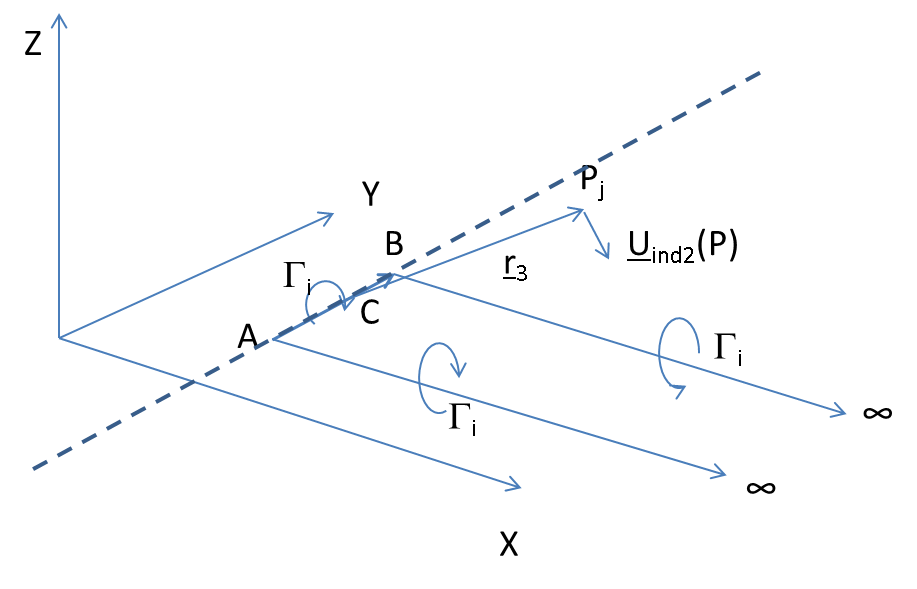
\includegraphics[width=0.8\linewidth]{PICS/inducedvel2}
	\caption{Contribution of the generic \emph{i-th} \gls{2d} bound vorticity to the induced velocity at the generic \gls{ctlpj}.}
	\label{fig:inducedvel2}
\end{figure}
%
%
\begin{subequations}\label{eq:inducedvel2}
\begin{alignat}{3}
%\begin{equation}\label{eq:inducedvel2}
	\gls{uindvij} &=& \gls{uabv} + \gls{uainfv} +  \gls{ubinfv} - \gls{uab2dv} \label{eq:uindvij} \\
	\gls{uab2dv} &=& \left\{
	    \begin{array}{lr}
		   \dfrac{\gls{circi}}{2\pi} \frac{\gls{r0} \times \gls{r3}}{ \left| \gls{r0} \times \gls{r3}\right|^2} \gls{r0m} \gls{deltaij}  \label{eq:uab2dv}
%		     & \mathrm{if }\quad \dfrac{\left|\gls{r3} \times \gls{r0}\right|}{\gls{r0m}} > \gls{epscore2} \\
%		     \dfrac{\left|\gls{r3} \times \gls{r0} \right|}{\gls{r0m}\gls{epscore2}}\gls{uab2dvpp} & \mathrm{otherwise}  
		\end{array}
		 \right.
\end{alignat}
\end{subequations} 
%\end{equation}
%
where \gls{r3} is the \glsentrydesc{r3}; \gls{uab2dv} is the \glsentrydesc{uab2dv} and it is considered only for control point within the local vortex element; \gls{deltaij} is the \glsentrydesc{deltaij}. % \gls{uab2dvpp} is the \glsentrydesc{uab2dvpp}, which can be calculated as in Eq.~\eqref{eq:uab2dvpp}:
%
%\begin{equation}\label{eq:uab2dvpp}
%\renewcommand*{\arraystretch}{2.5}
%\begin{array}{lcl}
%\gls{uab2dvpp} & = & \dfrac{\gls{circi}}{2\pi} \frac{\gls{r0} \times \gls{r3p}}{\gls{r0m} \left| \gls{r0} \times \gls{r3p}\right|^2} \\
%
%\mathrm{with} & \gls{r3p} = \gls{rppn} + \gls{epscore2} \gls{corerad2}
%\end{array} 
%\end{equation}
%


The induced velocity is therefore calculated as the difference between a \gls{3d} and a \gls{2d} contribution. By doing so, Eq.~\eqref{eq:KJ} can be enforced at each control point where \gls{urel}, \gls{aoa}, and \gls{clad} are expressed in terms of \gls{circi}. The resulting nonlinear system of equations can then be solved with a numerical method, \eg Newton's solver.

%Finally, one more modification is added to the model. The control points are rotated about the leading edge of each airfoil to lie in the plane identified by the freestream velocity and the local tangent to the \gls{14c}. This modification is in line with teh work of \cite{drela2015}.
\begin{equation}\label{eq:uind}
\gls{uindv}\left(\gls{ctlpj}\right)  = \sum_{i=1}^{\gls{nelms}} \gls{uindvij} =\sum_{i=1}^{\gls{nelms}} \left[ \gls{uabv} + \gls{uainfv} +  \gls{ubinfv}  - \gls{uab2dv} \right]
\end{equation}

The presence of multiple lifting surfaces is simply given by the superposition of the induced velocities (see Eq.~\eqref{eq:uind}, which replaces the second in Eq.~\eqref{eq:unknowns}), \ie the induced velocity at the generic \gls{ctlpj} is calculated the same way as in Eq.~\eqref{eq:inducedvel2}, where the contribution of each $i-th$ horseshoe vortex must be taken into account from all lifting surfaces. 

Enforcing Eq.~\eqref{eq:KJ} at each control point (one per horseshoe vortex) renders a system of nonlinear equations, where the various terms can be calculated as a function of \gls{circv} as shown in Eq.~\eqref{eq:unknowns} and Eq.~\eqref{eq:inducedvel2}, with \gls{clad} calculated from an interpolation of the airfoil polar data. 
%___________________________________________________________________________ %
\section{\gls{kitevsm} additional theory}\label{sec:kitevsm}
The \gls{vsm} is the base tool to calculate the distribution of lift along the wing span. \gls{mbdyn}, however, will require a set of loads at the various nodes (\gls{hsep}) along the wings. 

With reference to Figure~\ref{fig:pistolesi}, the calculation of shear forces and torque moment (pitching moment) at each spanwise station is done as follows:

\begin{itemize}
	\item with local values of \gls{urel}, \gls{aoa}, \gls{c}, \gls{deltay} (\glsentrydesc{deltay}) calculate:
	\begin{align}
	 \gls{Fx}=0.5\cdot \gls{rhoair} \gls{urel}^2 \gls{c} \gls{deltay} \left[ \gls{clad} \cdot \cos{\gls{aoa}} + \gls{cdad}  \cdot \sin{\gls{aoa}} \right] \label{eq:Fx}\\ 
	 \gls{Fy}=0.5\cdot \gls{rhoair} \gls{urel}^2 \gls{c} \gls{deltay} \left[- \gls{clad} \cdot \sin{\gls{aoa}} + \gls{cdad}  \cdot \cos{\gls{aoa}} \right] \label{eq:Fy} \\
	\gls{Mz}=0.5\cdot \gls{rhoair} \gls{urel}^2 \gls{c}^2  \gls{deltay}  \cdot \gls{cmad} 	 \label{eq:Mz}
	\end{align}
\end{itemize}

where \gls{clad}, \gls{cdad}, \gls{cmad} are given by interpolation of the airfoil tables (\gls{afi_params}). Note that these forces and moments are considered applied at the \gls{14c} points.

%___________________________________________________________________________ %
	
\chapter{Implementation Algorithm}\label{sec:implementation}
Here is a suggested approach to the algorithm implementation within \gls{fast8}.
%
%
\section{Inputs, Outputs, Parameters, States} \label{sec:uxyzp}
% ___________________________________________________________________ %
	\subsection{Init\_Inputs}\label{sec:init_inputs}

	Beside the standard variables common to all modules (\gls{outfmt}, \gls{outsfmt}, \gls{numouts}, \gls{outlist}),	the Init\_Inputs to the \gls{kitevsm} are:
	\begin{itemize}
		\item \gls{vsmmod} --\glsentrydesc{vsmmod} 
		DOES THIS ONE GO IN TO KiteAD?
		
		\item \gls{deltay}: \glsentrydesc{deltay} per element
		\item \gls{c}: \glsentrydesc{c} per wing element
		
		\item \gls{afidx}: \glsentrydesc{afidx} per wing element
		\item \gls{twistaer}: per wing element

		%\item \gls{hsep}: \glsentrydesc{hsep} at \gls{t0}
		%\item \gls{ctlp}: \glsentrydesc{ctlp} at \gls{t0}	
	\end{itemize}
	
Do all the calculations the first time CalcOutput is called setting a temporary variable that mimics the sate.
	%
	% ___________________________________________________________________ %
	\section{Inputs u}\label{sec:inputs}
	The Inputs to the \gls{kitevsm} are:
	\begin{itemize}
		\item \gls{uoov}: \glsentrydesc{uoov}. What is really needed are the components in the plane of the local element airfoil (\gls{xaxis}, \gls{yaxis}), including contributions from structural body motions and wind velocity.

		\item \gls{A},\gls{B} coordinates for every element, in the aircraft reference frame \gls{xyzb}. From these, the local chord length, and the \gls{uoov}, the \gls{hsep} and \gls{ctlp} coordinates can be calculated. 
		\item \gls{twist}: \glsentrydesc{twist} per wing element
	
		\item \gls{df}: \glsentrydesc{df} (control setting per blade element)	

	\end{itemize}
	Note: these are for a given node (within a given lifting surface) and chord. Density is used to calculate the dimensional load at each spanwise station.
	\gls{uoo} should include the body motion.
	% ___________________________________________________________________ %		
	\section{Outputs y}\label{sec:outputs}
	The Outputs from the \gls{kitevsm} are:
	\begin{itemize}
		\item \gls{Fx}: \glsentrydesc{Fx}
    	\item \gls{Fy}: \glsentrydesc{Fy}
		\item \gls{Mz}: \glsentrydesc{Mz}

						
	\end{itemize}
	The outputs are calculated via Eqs.~\eqref{eq:Fx}--\eqref{eq:Mz}, and using Eqs.~\eqref{eq:unknowns} with the calculated state \gls{circi}.
	%Note: \gls{kitevsm} will need to integrate the \gls{cn}, \gls{cc}, \gls{cm} for any given wing element.
	% ___________________________________________________________________ %	
	\section{States \gls{xc}}\label{sec:states}
	The states for \gls{kitevsm} are constraint states:\newline
    %	
	\begin{itemize}
		\item \gls{circy}: \glsentrydesc{circy}
	\end{itemize}

	Note: perhaps normalizing \gls{circy} by the local \gls{uoov} could reduce errors in the residual within the \emph{CalcOutput} calculations where the new time step \gls{uoov} will be used.
	% ___________________________________________________________________ %	
	\section{Parameters p}\label{sec:parameters}
	The Parameters for the \gls{kitevsm} are:
	\begin{itemize}
				\item \gls{vsmmod} --\glsentrydesc{vsmmod} 
		DOES THIS ONE GO IN TO KiteAD?
		
		\item \gls{deltay}: \glsentrydesc{deltay} per element
		\item \gls{c}: \glsentrydesc{c} per wing element
		
	
		\item \gls{twistaer}: per wing element
		
		\item \gls{afi_params}: \glsentrydesc{afi_params}
		\item \gls{afidx}: \glsentrydesc{afidx}
		\item \gls{airvisc}: \glsentrydesc{airvisc}
	\end{itemize}
				
	%__________________________________________________________________ %
	\section{\Acrlong{kitevsm} Implementation}
		
		
	\subsection{\glstext{kitevsm}\_Init Routine}
	This routine allocates the module's data structures, initializes the module's states, and sets the non-time-varying  parameters (copies them from the initialization input data section) (see also Section~\ref{sec:init_inputs}).
	\begin{itemize}
		\item \gls{circy}(0)= elliptical distribution
	\end{itemize}
	
	
	\subsection{\glstext{kitevsm}\_UpdateStates Routine}
		
	For a given set of inputs (u), and at the current step in time ($\gls{t}_i$): 
	\begin{itemize}
		\item	use the current time step $\gls{circy}_{i}$ as initial guess to solve for $\gls{circy}_{i+1}$ by numerically solving Eq.~\eqref{eq:KJ}, together with Eqs.~\eqref{eq:3dindvel},~\eqref{eq:inducedvel2}, and \eqref{eq:unknowns}. Inputs will come in at $\gls{t}_{i+1}$

	\end{itemize}	
%	
    
%_________________________________________________________ %			
%
		 		 		
	\subsection{\glstext{kitevsm}\_CalcOutput}

	By using Eqs.\eqref{eq:Fx}--\eqref{eq:Mz}, calculate:
	%
    \begin{itemize}
       \item \gls{Fx}: \glsentrydesc{Fx}
       \item \gls{Fy}: \glsentrydesc{Fy}
       \item \gls{Mz}: \glsentrydesc{Mz}
    \end{itemize}	

The outputs are calculated via Eqs.~\eqref{eq:Fx}--\eqref{eq:Mz}, and using Eqs.~\eqref{eq:unknowns} with the calculated state \gls{circi} through Eqs.~\eqref{eq:3dindvel}, \eqref{eq:uabinfvpp}, \eqref{eq:uabvpp}, \eqref{eq:inducedvel2}, and \eqref{eq:uab2dvpp}.
%_________________________________________________________%	

% bibliography
\cleardoublepage
\label{sec:Bib}
%\bibliography{C:/RRD/LITERATURE/references} %local natbib file
\printbibliography
\end{document}